% Simulaing Neutrino Oscillation Experiments with GLoBES
% -----------------------------------------------------------------------------
% Talk given at the 2005 Ringberg Young Scientists Workshop on Hot
% Topics in Particle and Astroparticle Physics
% -----------------------------------------------------------------------------
\documentclass{beamer}

% -----------------------------------------------------------------------------
\title[Neutrino Oscillations and GLoBES]
      {Simulating Neutrino Oscillation Experiments with GLoBES}
\author[J. Kopp, A. Merle]
       {\parbox{9 cm}{Part 1: Alexander Merle (\texttt{amerle@ph.tum.de}) \\
                      -- Theory of Neutrino Oscillations       \\
                      -- State of the Art in Neutrino Physics  \\ \\
                      Part 2: Joachim Kopp (\texttt{jkopp@ph.tum.de})     \\
                      -- The GLoBES Software Package           \\
                      -- Simulation of Future Experiments}}
\institute[TUM]
          {TU M\"unchen, Lehrstuhl T30d f\"ur Theoretische Elementarteilchenphysik (Prof. Lindner)}
\date[21.07.2005]
     {Young Scientists Workshop on Hot Topics in Particle and Astroparticle Physics \\
      18.07. - 22.07.2005, Ringberg Castle}
% -----------------------------------------------------------------------------
\usepackage[english]{babel}
\usepackage{times}
\usepackage[T1]{fontenc}
\usepackage{amsmath}
\usepackage{graphicx}

% Set up beamer package
\mode<presentation>
{
  \usetheme{Madrid}
  \setbeamercovered{transparent}
}
\setbeamertemplate{navigation symbols}{}


% Some commands to simplify things
\newcommand{\twovec}[2]{\ensuremath{ \left( \begin{array}{c} {#1}\\{#2} \end{array} \right) }}
\newcommand{\twomat}[4]{\ensuremath{ \left( \begin{array}{lr} {#1} & {#2} \\ {#3} & {#4} \end{array} \right) }}
\newcommand{\threevec}[3]{\ensuremath{ \left( \begin{array}{c} {#1}\\{#2}\\{#3} \end{array} \right) }}
\newcommand{\threemat}[9]{\ensuremath{ \left( \begin{array}{lcr} {#1} & {#2} & {#3} \\
                                                                {#4} & {#5} & {#6} \\
                                                                {#7} & {#8} & {#9} \end{array} \right) }}
\newcommand{\degrees}{\ensuremath{^\circ}}
\newcommand{\reference}[1]{\tiny #1 \normalsize}


% Show table of content before each section
\AtBeginSection[]
{
    \begin{frame}
      \frametitle{Outline}
      \tableofcontents[currentsection]
    \end{frame}
}


\begin{document}

\begin{frame}
  \titlepage
\end{frame}


\begin{frame}
  \frametitle{Outline}
  \tableofcontents
\end{frame}


% =============================================================================
\section{The Neutrino Oscillation Framework}
% =============================================================================

%..............................................................................
\subsection{2-Flavour Oscillations in Vacuum}
% -----------------------------------------------------------------------------

\begin{frame}
  \frametitle{Mass and flavour eigenstates}

  \begin{itemize}
    \item For neutrinos, the eigenstates of the mass operator are not equal to
    the ones of the weak interaction:
    
   \begin{figure}
    \begin{center}
      \includegraphics[width=7.5cm]{fig/osc1.jpg}
    \end{center}
  \end{figure}
        
     \item  Massless neutrinos: the mass eigenstates can be arbitrarily chosen $\Rightarrow$ can be defined as identical to the flavour eigenstates $\Rightarrow$ no oscillations! $\Rightarrow$ oscillations are the evidence for non-zero neutrino mass!  

   \end{itemize}
\end{frame}


\begin{frame}
  \frametitle{The formalism}

  \begin{itemize}
    \item Let ($|\nu_{e}\rangle$,$|\nu_{\mu}\rangle$) be the flavour and ($|\nu_1\rangle$,$|\nu_2\rangle$) the mass eigenstates $\Rightarrow$ every flavour-state can be written as a linear combination of mass eigenstates (since it is a rotation one can use a rotation matrix):

$$
\left(\begin{array}{c}
| \nu_{e} \rangle \\
| \nu_{\mu} \rangle \\
\end{array}\right)
=
\left(\begin{array}{cc}
\cos \theta & \sin \theta\\
-\sin \theta	& \cos\theta\\
\end{array}\right)
\cdot
\left(\begin{array}{c}
| \nu_{1} \rangle \\
| \nu_{2} \rangle \\
\end{array}\right)
$$
    
	\item Time evolution: $$|\nu_{e} (t) \rangle \ =\ \cos \theta  \ e^{-iE_1 t}|\nu_1 (t=0) \rangle \ + \ \sin \theta \ e^{-iE_2 t}|\nu_2 (t=0) \rangle $$

	\item Energy momentum relation: $$E_{i}^2=p_{i}^2+m_{i}^2 \Rightarrow E_{i}=\sqrt{p_{i}^2 +m_{i}^2}\approx p_{i}+\frac{m_{i}^2}{2p_{i}}$$
    

   \end{itemize}
\end{frame}



\begin{frame}
  \frametitle{Diasappearance Probability}

  \begin{itemize}
    \item Assumption: both of the mass eigenstates have the same momentum p (in fact, this does not have to be true, but the longer calculation gives the same result) $\Rightarrow$ with $p=E_{\nu}$: $E_2=E_1-\frac{\Delta m^2}{2E_{\nu}}$ where $\Delta m^2 =m_1^2 - m_2^2$

	\item E. g. for the muon-neutrino we get: $$|\nu_{\mu} \rangle =e^{-i(p+\frac{m_{1}^2}{2p})t} \cdot \left[ -\sin\theta \ |\nu_1(0) \rangle +\cos\theta \ e^{\frac{i\Delta m^2}{2E_{\nu}}} |\nu_2(0) \rangle \right]$$
    
	\item With a simple calculation (trigonometric identities, etc.) one can construct the probability for detecting a $\nu_{\mu}$ as a $\nu_e$ at a time t: $$P_{\nu_{\mu}\rightarrow \nu_{e}}(t)=| \langle \nu_{e}(0)|\nu_{\mu}(t) \rangle |^2=|(\cos\theta \ \langle \nu_1(0)| + \sin \theta \ \langle \nu_2(0)| ) \cdot |\nu_{\mu}(t) \rangle |^2$$ $=\sin^2 (2\theta) \cdot \sin^2 (\frac{t \Delta m^2}{4E_{\nu}} ) \Rightarrow$ oscillates with time!  
   

   \end{itemize}
\end{frame}



\begin{frame}
  \frametitle{Survival Probability}

  \begin{itemize}
    \item Probability to see the $\nu_{\mu}$ again as a $\nu_{\mu}$: $$P_{\nu_{\mu}\rightarrow \nu_{\mu}}(t)=1-P_{\nu_{\mu}\rightarrow \nu_{e}}(t)=1-\sin^2 (2\theta) \cdot \sin^2 (\frac{t \Delta m^2}{4E_{\nu}} )$$ 

	\item Neutrinos travel (nearly) with the speed of light $\Rightarrow$ one can set t=x, where x is the distance to the place where the neutrino was born

	\item Oscillation length: distance after which the $\nu_{\mu}$ is again a 100 \% $\nu_{\mu}$ $$ \sin^2(\frac{x \Delta m^2}{4E_{\nu}})\equiv \sin^2(\frac{\pi x}{L_0}) \Rightarrow L_0=\frac{4\pi E_{\nu}}{\Delta m^2} \propto \frac{E_{\nu}}{\Delta m^2}$$ 
   $\rightarrow$ important quantity for experiments

	\item Notice, that only the squared mass difference $\Delta m^2$ can be determined by oscillation experiments!

   \end{itemize}
\end{frame}


% -----------------------------------------------------------------------------
\subsection{Matter Effects}
% -----------------------------------------------------------------------------

\begin{frame}
  \frametitle{Matter Effects}

  \begin{itemize}
 	\item The Hamiltonian in the basis of the mass eigenstates is diagonal $\Rightarrow$ Schr\"odinger's equation (one can skip the first p from $E=p+\frac{m^2}{2p}$ since it just gives a global phase): 
$$
i\frac{d}{dt}
\left(\begin{array}{c}
| \nu_{1} \rangle \\
| \nu_{2} \rangle \\
\end{array}\right)=
H_{M}
\left(\begin{array}{c}
| \nu_{1} \rangle \\
| \nu_{2} \rangle \\
\end{array}\right)=
\frac{1}{2p}\cdot
\left(\begin{array}{cc}
m_1^2 & 0\\
0 & m_2^2\\
\end{array}\right)
\left(\begin{array}{c}
| \nu_{1} \rangle \\
| \nu_{2} \rangle \\
\end{array}\right)$$

	\item To go into the flavour basis, one has to rotate the states as well as the Hamiltonian by a unitary matrix U, which leeds to the Hamiltonian $H_{F}$ in the flavour basis:
$$
H_{F}=
\frac{1}{2p}\cdot
\left(\begin{array}{cc}
m_{ee}^2 & m_{e \mu}^2\\
m_{e \mu}^2 & m_{\mu \mu}^2\\
\end{array}\right)=
U H_{M} U^{\dagger}=
$$
$$
=\frac{1}{2p} \cdot
\left(\begin{array}{cc}
\cos \theta & \sin \theta\\
-\sin \theta & \cos \theta\\
\end{array}\right)
\cdot
\left(\begin{array}{cc}
m_1^2 & 0\\
0 & m_2^2\\
\end{array}\right)
\cdot
\left(\begin{array}{cc}
\cos \theta & -\sin \theta\\
\sin \theta & \cos \theta\\
\end{array}\right)=
$$

 
  \end{itemize}
\end{frame}




\begin{frame}
  \frametitle{Matter Effects}

$$
=\frac{1}{4p}\left[ \Sigma 
\left(\begin{array}{cc}
1 & 0\\
0 & 1\\
\end{array}\right)
+D
\left(\begin{array}{cc}
-\cos(2 \theta) & \sin(2 \theta)\\
\sin(2 \theta) & \cos(2 \theta)\\
\end{array}\right)
\right]
$$	
  
\hspace{2cm} where $\Sigma=m_1^2+m_2^2$ and $D=m_2^2-m_1^2$
 
  \begin{itemize}

	\item Since it is diagonal, the first term just gives a common phase $\Rightarrow$ has no physical meaning

	\item Coherent forward scattering in matter: $\nu_e$ and $\overline{\nu}_e$ can - different from all other flavours - interact with the electrons via CC-reactions $\Rightarrow$ change of the oscillation probabilities!

	\item The Hamiltonian in the flavour basis has to be changed: 
$$H_{F} \rightarrow H_{F, mat}=H_{F}+\frac{1}{2p}
\left(\begin{array}{cc}
A & 0\\
0 & 0\\
\end{array}\right)$$
where $A=2\sqrt{2}G_{F}N_{e}p$ ($G_F$: Fermi's constant, $N_e$: electron density)
    
  \end{itemize}
\end{frame}



\begin{frame}
  \frametitle{Matter Effects}

  \begin{itemize}
    \item Back to the mass eigenstates $\Rightarrow$ after a lengthy calculation we get:
$$
H_{M,mat}=
\frac{1}{2p} \cdot
\left(\begin{array}{cc}
m_1^2+A \cos^2(\theta) & A \sin(\theta) \cos(\theta)\\
A \sin(\theta) \cos(\theta) & m_2^2+A \sin^2(\theta)\\
\end{array}\right)
$$

$\Rightarrow$ this Hamiltonian is not diagonal anymore $\Rightarrow$ the mass eigenstates of the vacuum are not eigenstates in matter 

	\item So one has to diagonalize again to get the new mass eigenstates $|\nu_{1m}\rangle$ and $|\nu_{2m}\rangle$ in matter, which gives

$$m_{1,2m}^{2}=\frac{1}{2}\cdot \left[ (\Sigma + A) \pm \sqrt{(A-D \cos(2 \theta))^2+ D^2 \sin^2(2\theta)} \right]$$ 

and so the squared mass difference in matter is (remember that $D=m_2^2-m_1^2$)

$$D_{m}=m_{2m}^{2}-m_{1m}^{2}= D \cdot \sqrt{(\frac{A}{D}-\cos(2 \theta))^2+\sin^2(2 \theta)}$$


   \end{itemize}
\end{frame}




\begin{frame}
  \frametitle{Matter Effects}

  \begin{itemize}
    \item So we also have in matter a new mixing angle $\theta_{mat}$
and so a new transition probability
$$P_{mat, \nu_e \rightarrow \nu_{\mu}}(x)= \sin^2(2\theta_{mat}) \sin^2\left(\frac{x D_{m}}{4p}\right) $$

	\item The oscillation amplitude is

$$\sin^2(2\theta_{mat})=\frac{\sin^2(2 \theta)}{(\frac{A}{D}-\cos(2 \theta))^2+\sin^2(2 \theta)}=f(A/D)=f(E_{\nu}N_e)$$
$\Rightarrow$ the ratio $\frac{A}{D}$ determines the oscillation probabilities in matter $\Rightarrow$ for $\frac{A}{D}\approx\cos(2\theta)$ we have a resonance effect $\Rightarrow$ \textbf{a muon-neutrino can at certain distances be a 100\% electron-neutrino!!!} 

   \end{itemize}
\end{frame}


\begin{frame}
  \frametitle{Flavour-Flipping/The MSW-Effect}

(\underline{M}ikheyev-\underline{S}mirnov-\underline{W}olfenstein)

\begin{figure}
    \begin{center}
      \includegraphics[width=7.5cm]{fig/resonant.jpg}
    \end{center}
  \end{figure}

e.g. the first mass eigenstate ($\nu_{1m}$-curve) is most probably a $\nu_e$ below and most probably a $\nu_{\mu}$ above the resonant matter density $A_R$
  
\end{frame}

%..............................................................................
\subsection{3-Flavour Oscillations }
%..............................................................................


\begin{frame}
  \frametitle{3-Flavour Oscillations}
	\begin{itemize}

	\item For 3 neutrino-flavours the mixing looks like:
$$
\left(\begin{array}{c}
| \nu_{e} \rangle \\
| \nu_{\mu} \rangle \\
| \nu_{\tau} \rangle \\
\end{array}\right)=
U\cdot
\left(\begin{array}{c}
| \nu_{1} \rangle \\
| \nu_{2} \rangle \\
| \nu_{3} \rangle \\
\end{array}\right)
$$
with $U^{\dagger}=U^{-1}$ and
$$
U=
\left(\begin{array}{ccc}
c_{12}c_{13} & s_{12}c_{13}&s_{13}e^{-i\delta}\\
-s_{12}c_{23}-c_{12}s_{23}s_{13}e^{i\delta} & c_{12}c_{23}-s_{12}s_{23}s_{13}e^{i\delta} & s_{23}c_{13}\\
s_{12}s_{23}-c_{12}c_{23}s_{13}e^{i\delta} & -c_{12}s_{23}-s_{12}c_{23}s_{13}e^{i\delta} & c_{23}c_{13}\\
\end{array}\right)
$$
where c$_{ij}=\cos(\theta_{ij})$ and s$_{ij}=\sin(\theta_{ij})$

\item Parameters: 3 mixing angles ($\theta_{12}$, $\theta_{23}$ and $\theta_{13}$), 1 CP-violating phase ($\delta$) and 2 squared mass differences ($(\Delta m^2)_{sol}=(\Delta m^2)_{21}$ and $(\Delta m^2)_{atm}=(\Delta m^2)_{31}$)

	\end{itemize}  
\end{frame}



\begin{frame}
	\frametitle{3-Neutrino-Mixing}

\begin{figure}
    \begin{center}
      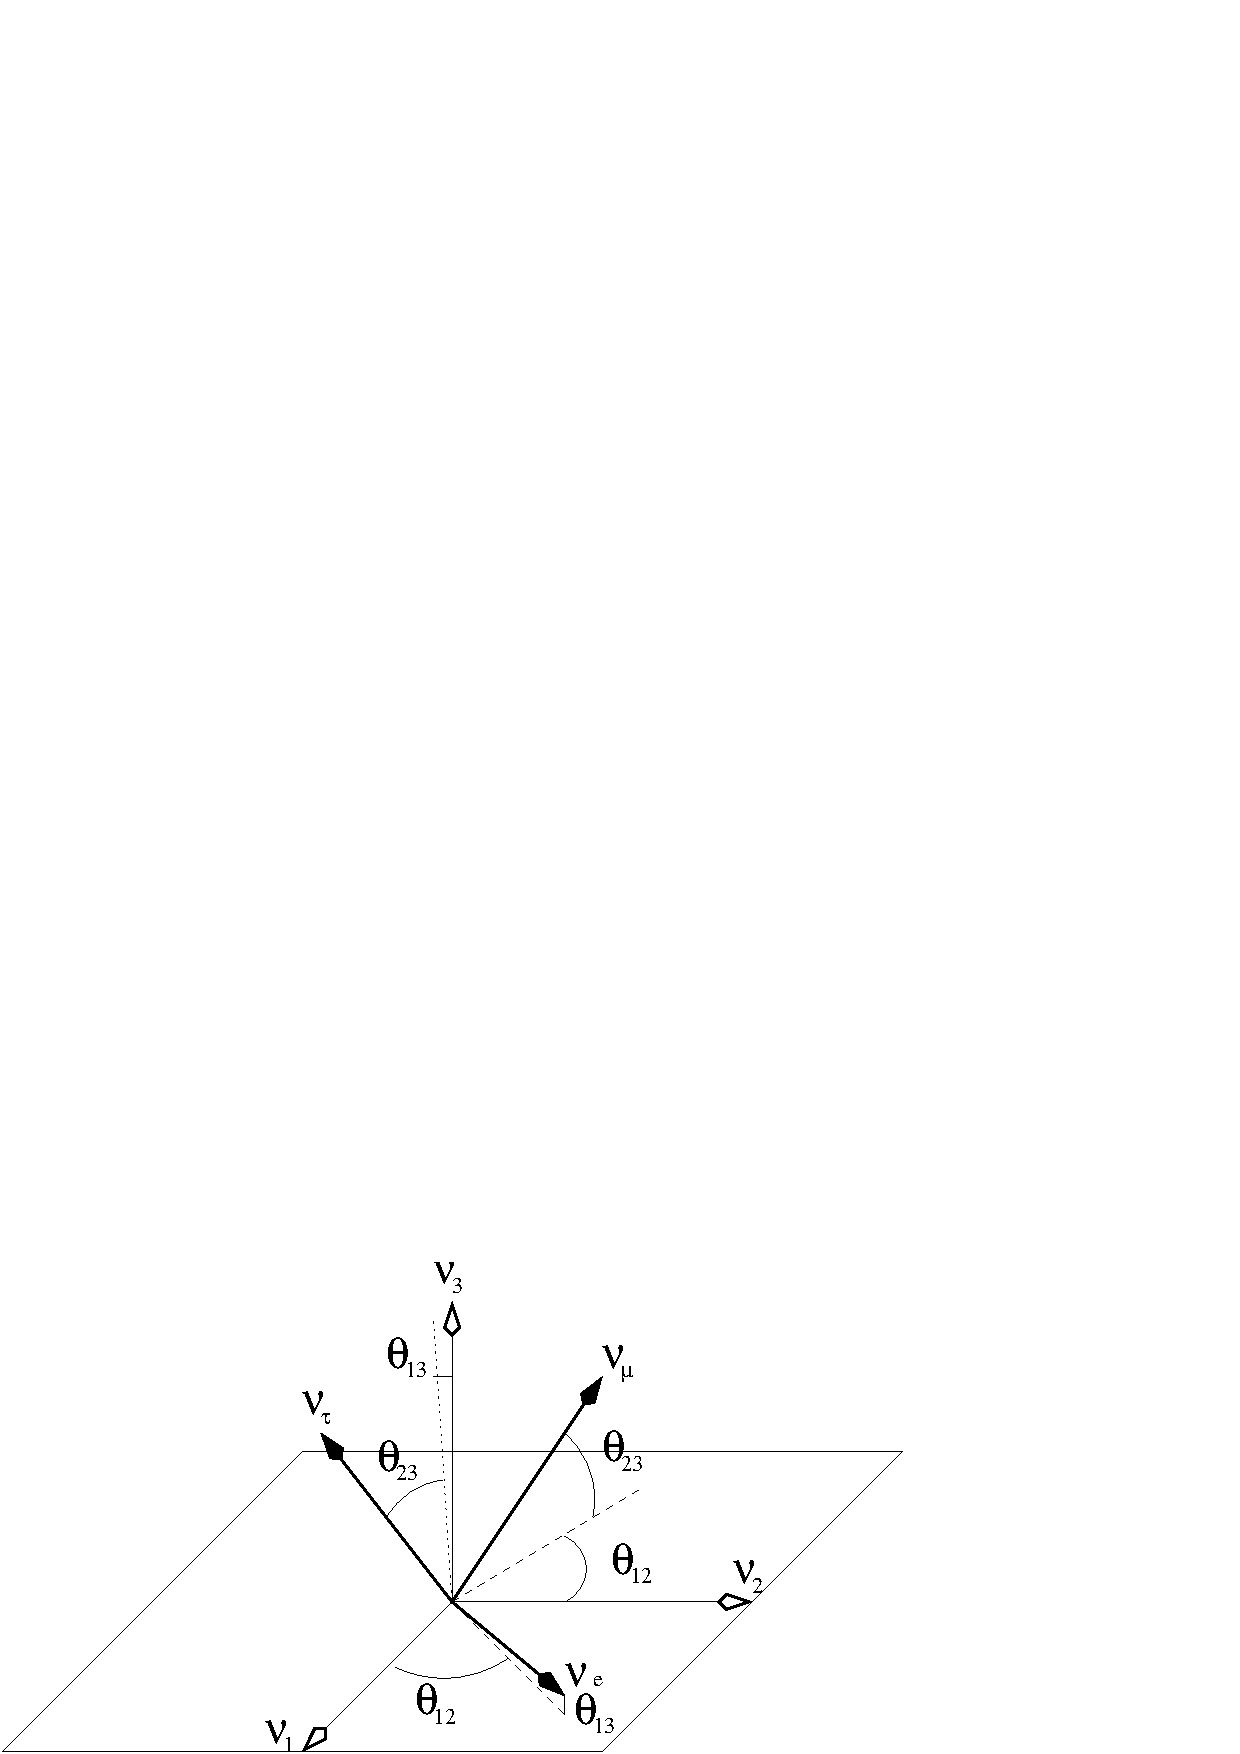
\includegraphics[width=12cm]{fig/angles.pdf}
    \end{center}
 \end{figure}


\end{frame}



% =============================================================================
\section{The State of the Art in Neutrino Physics}
% =============================================================================

%..............................................................................
\subsection{The Oscillation Parameters}
% -----------------------------------------------------------------------------
\begin{frame}
	\frametitle{The Oscillation Parameters}

\begin{block}{}
    \begin{tabular}{lcc}
      Parameter         &  Best fit value and $\pm 3 \sigma$ range & Experiments \\ \hline \\ 
	$\theta_{12}\approx 32.6\degrees $		&  $\sin^2(\theta_{12})=0.29^{+0.08}_{-0.06}$	 & solar/reactor neutrinos \\ 
	$\theta_{23}\approx 45.0\degrees$ 		&  $\sin^2(\theta_{23})=0.50\pm 0.16$		&   atmospheric/accelerator\\
	$\theta_{13}\lesssim 9.6\degrees$ 		& $\sin^2(\theta_{13})=0.000+0.047$ & CHOOZ-experiment\\
	\hspace{0.8cm}$\delta$			 & ????? & several proposals\\
	\hspace{0.3cm}$(\Delta m^2)_{21}$  & $(8.1^{+1.0}_{-0.8})\cdot 10^{-5}$ eV$^2$ & solar/reactor\\
	\hspace{0.3cm}$(\Delta m^2)_{31}$  & $(2.2^{+1.1}_{-0.8}) \cdot 10^{-3}$ eV$^{2}$ & atmospheric/accelerator\\
	\end{tabular}
\begin{flushright}
\tiny{taken from Maltoni, Schwetz et al., New J. Phys. 6 (2004)\\
see also: Bahcall et al., JHEP 08 (2004) or Bandyopadhyay et al., Phys. Lett. B608 (2005)}
\end{flushright}
	 \end{block}

\begin{itemize}
    \item
    Two large mixing angles and one small mixing angle ($\neq$CKM!).

    \item
    No information about CP violation.

    \item
    Precise measurement of neutrino mixing parameters is essential for a deeper
    theoretical understanding of flavour physics and physics beyond the Standard Model.
  \end{itemize}


\end{frame}



%..............................................................................
\subsection{Mass Hierarchies}
%..............................................................................
\begin{frame}
	\frametitle{Mass Hierarchies}

Problem: since oscillation only measures squared mass differences, and we do not know the sign of $(\Delta
m^2)_{atm}$ yet, there could be different hierarchies


\begin{figure}
    \begin{center}
      \includegraphics[width=8cm]{fig/hierarchy.pdf}
    \end{center}
 \end{figure}

$\Rightarrow$ from the oscillations we get only the information, that neutrinos do have mass, but nothing about the absolute values

\end{frame}


% -----------------------------------------------------------------------------
\subsection{The Past and the Future}
% -----------------------------------------------------------------------------


\begin{frame}
	\frametitle{Where do we know all that from?}

\begin{itemize}

\item Super-Kamiokande (atmospheric $\nu$'s), K2K,... $\Rightarrow$ $\theta_{23}$, $(\Delta m^2)_{31}$
\begin{figure}
    \begin{center}
      \includegraphics[width=3.8cm]{fig/atm1.jpg}
    \end{center}
 \end{figure}

\item Solar neutrinos, KamLAND, ... $\Rightarrow$ $\theta_{12}$, $(\Delta m^2)_{21}$
\begin{figure}
    \begin{center}
      \includegraphics[width=3cm]{fig/sun.jpg}
    \end{center}
 \end{figure}

\item CHOOZ $\Rightarrow$ $\theta_{13}$

\end{itemize}

\end{frame}



\begin{frame}
\frametitle{The next steps}

\begin{itemize}
\item Achieving a better precision for the known mixing parameters
\item Measurement of the small mixing angle $\theta_{13}$
\item Measurement of the CP-phase $\delta$
\end{itemize}

\vspace{1.5cm}

\large{AND (what we do): Making Simulations with GLoBES }
\end{frame}



% =============================================================================
\section{GLoBES - The General Long Baseline Experiment Simulator}
% =============================================================================

% -----------------------------------------------------------------------------
\subsection{GLoBES Basics}
% -----------------------------------------------------------------------------

\begin{frame}
  \frametitle{The GLoBES software package}

  \begin{columns}
    \begin{column}{6 cm}
      \begin{figure}
        \includegraphics[width=5 cm]{fig/globes_logo.jpg}
      \end{figure}
    \end{column}
    \begin{column}{6 cm}
      \begin{itemize}
        \item C library for simulating neutrino oscillation experiments
        \item Provides sophisticated functions for high level and low level access
              to the simulation
        \item AEDL --- Abstract Experiment Definition Language for defining experimental
              setups
        \item Developed at TUM by P.~Huber, M.~Lindner and W.~Winter \\
      \end{itemize}
    \end{column}
  \end{columns}
  \begin{flushright}
    \reference{Comput. Phys. Commun. 167:195, 2005, hep-ph/0407333}
  \end{flushright}
\end{frame}


\begin{frame}
  \frametitle{Components of a GLoBES simulation}

  \begin{columns}
    \begin{column}{5.5 cm}
      \begin{block}{Neutrino Sources}
        \parbox[t][2.6 cm]{5.2 cm}{  
        \begin{itemize}
          \item Energy and flavour spectrum
          \item Signal and Background
        \end{itemize}}
      \end{block}
      \begin{block}{Detector}
        \parbox[t][2.7 cm]{5.2 cm}{  
        \begin{itemize}
          \item Interaction cross sections
          \item Energy resolution
          \item Systematical errors
        \end{itemize}}
      \end{block}
    \end{column}
    \begin{column}{5.5 cm}
      \begin{block}{Oscillations}
        \parbox[t][2.6 cm]{5.2 cm}{  
        \begin{itemize}
          \item Fundamental parameters: $\theta_{12}$, $\theta_{13}$, $\theta_{23}$,
                $\delta$, $\Delta m_{21}^2$, $\Delta m_{31}^2$.
          \item Baseline and matter density profile
        \end{itemize}}
      \end{block}
      \begin{block}{Analysis}
        \parbox[t][2.7 cm]{5.2 cm}{  
        \begin{itemize}
          \item Number and width of energy bins
          \item Fitting parameters to the simulated data
          \item $\chi^2$ analysis
        \end{itemize}}
      \end{block}
    \end{column}
  \end{columns}
\end{frame}

\begin{frame}
  \frametitle{Calculation of event rates}
  \begin{block}{}
    \vspace{-0.2 cm}
    \begin{eqnarray*}
      \frac{dn_{f}^{\mathrm{IT}}}{dE'} &\propto&  \sum_{f_i}\int \int dE\,d\hat{E}\quad
                              \underbrace{\Phi_{f_i} (E)}_{\mathrm{Production}} \times \\
            &&\underbrace{\frac{1}{L^2} P_{(f_i\rightarrow f)}(E,L,\rho;\theta_{23},\theta_{12},\theta_{13},
                     \Delta m^2_{31},\Delta m^2_{21},\delta)}_{\mathrm{Propagation}}
                     \times \nonumber \\ &&\underbrace{\sigma^{\mathrm{IT}}_f(E)
                         k_f^{\mathrm{IT}}(E-\hat{E})}_{\mathrm{Interaction}} \times 
              \underbrace{ T_f(\hat{E}) V_f(\hat{E}-E')}_{\mathrm{Detection}}
    \end{eqnarray*}
    \begin{flushright}
      \reference{P. Huber, M. Lindner, W. Winter, Nucl. Phys. B645:3-48, 2002, hep-ph/0204352}
    \end{flushright}
  \end{block}
  \small
  \begin{tabular}{l@{\ }c@{\ }ll@{\ }c@{\ }l}
    $E$              &=& Neutrino energy       & $P_{(f_i\rightarrow f)}(\ldots)$ &=& Oscillation probability      \\
    $\hat{E}$        &=& Charged Lepton energy & $\sigma^{\mathrm{IT}}_f(E)$      &=& Cross sections               \\
    $E'$             &=& Reconstructed energy  & $k_f^{\mathrm{IT}}(E-\hat{E})$   &=& Charged lepton distribution  \\
    $\Phi_{f_i} (E)$ &=& Source flux           & $T_f(\hat{E})$                   &=& Threshold function           \\
    $L$              &=& Baseline              & $V_f(\hat{E}-E')$                &=& Energy resolution function
  \end{tabular}
\end{frame}


\begin{frame}
  \frametitle{Sensitivity of a reactor experiment to $\sin^2 (2 \theta_{13})$}

  \begin{enumerate}
    \item Define what you want to measure: What 90 \% C.L. limit can the experiment set on
          $\sin^2 (2 \theta_{13})$, assuming the true value is 0?
    \item Define the setup using AEDL (Abstract Experiment Definition Language)
    \item Calculate the ``true'' event rates.
    \item Now calculate the expected event rates for nonzero values of $\sin^2 (2 \theta_{13})$.
    \item Perform a $\chi^2$ analysis to find out which values produce event rates that
          are still compatible with $\sin^2 (2 \theta_{13}) = 0$ at the chosen C.L.
  \end{enumerate}
\end{frame}


% -----------------------------------------------------------------------------
\subsection{$\chi^2$ Analysis}
% -----------------------------------------------------------------------------

\begin{frame}
  \frametitle{$\chi^2$ Analysis in GLoBES}

  \begin{tabular}{ll}
    \begin{minipage}[b]{6 cm}
      \begin{itemize}
        \item
        If $X_i$ are normally distributed with $\langle X_i \rangle = 0$ and $\sigma = 1$,
        then $\chi^2 = \sum_{i=1}^n X_i^2$ is distributed according to the $\chi^2$
        distribution with $n$ degrees of freedom.
      \end{itemize}
      \vspace{0.2 cm}
    \end{minipage}    &
    \includegraphics[height=3 cm]{fig/chi2_dist.pdf} \\

    \multicolumn{2}{l}{
    \begin{minipage}{10 cm}
      \begin{itemize}
        \item
        For $n$ energy bins with event rates following the Poisson distribution
        \vspace{-0.3 cm}
        \begin{equation*}
          \chi^2 = \sum_{i=1}^n 2 (N_i(\vec{\Lambda}) - N_i(\vec{\Lambda}_0))
                          + 2 N_i(\vec{\Lambda}) \log \frac{N_i(\vec{\Lambda})}{N_i(\vec{\Lambda}_0)}
          \vspace{-0.2 cm}
        \end{equation*}
        follows a $\chi^2$ distribution with $\dim \vec{\Lambda}$ degrees of freedom. Here: \\
        \vspace{0.3 cm}
        \begin{tabular}{lcl}
          $N_i(\vec{\Lambda}_0)$ &=& Event rates for true parameter values $\vec{\Lambda}_0$.  \\
          $N_i(\vec{\Lambda})$   &=& Event rates for hypothesised parameters $\vec{\Lambda}$.
        \end{tabular}
      \end{itemize}
    \end{minipage}}
  \end{tabular}
\end{frame}


\begin{frame}
  \frametitle{$\chi^2$ Analysis in GLoBES}
  \begin{block}{Inclusion of systematics and external input}
    \begin{eqnarray*}
      \chi^2 &=& \underbrace{\sum_{i=1}^n 
                    2 (N_i(\vec{\Lambda},\vec{x}) - N_i(\vec{\Lambda}_0,\vec{x}_0))
                          + 2 N_i(\vec{\Lambda},\vec{x})
                                   \log \frac{N_i(\vec{\Lambda},\vec{x})}{N_i(\vec{\Lambda}_0,\vec{x}_0)}}
                           _{\textnormal{Statistical part}}   \\
          && + \ \ \ \underbrace{\sum_{j=1}^{\dim{\vec{\Lambda}}}
                   \frac{(\vec{\Lambda}_j - \vec{\Lambda}_{0j})^2}{\sigma_{\vec{\Lambda}j}^2}}
                           _{\textnormal{External input}} \ \ \
             + \ \ \ \underbrace{\sum_{k=1}^{\dim{\vec{x}}} \frac{(\vec{x}_k - \vec{x}_{0k})^2}{\sigma_{\vec{x}k}^2}}
                           _{\textnormal{Systematics}}
    \end{eqnarray*}
  \end{block}
  \small
  \begin{tabular}{lcl}
    $\vec{\Lambda}, \vec{\Lambda}_0$  &=& True and hypothesised oscillation parameters             \\
    $\vec{x}, \vec{x}_0$              &=& Systematics parameters                                   \\
    $N_i(\vec{\Lambda},\vec{x})$      &=& Expected event rates                                     \\
    $\sigma_{\vec{\Lambda}j}$         &=& Standard errors of external parameter input              \\
    $\sigma_{\vec{x}k}$               &=& Standard errors of systematics parameters 
  \end{tabular}
\end{frame}


\begin{frame}
  \frametitle{$\chi^2$ Analysis in GLoBES}
  
  \begin{figure}
    \raisebox{0.5 cm}{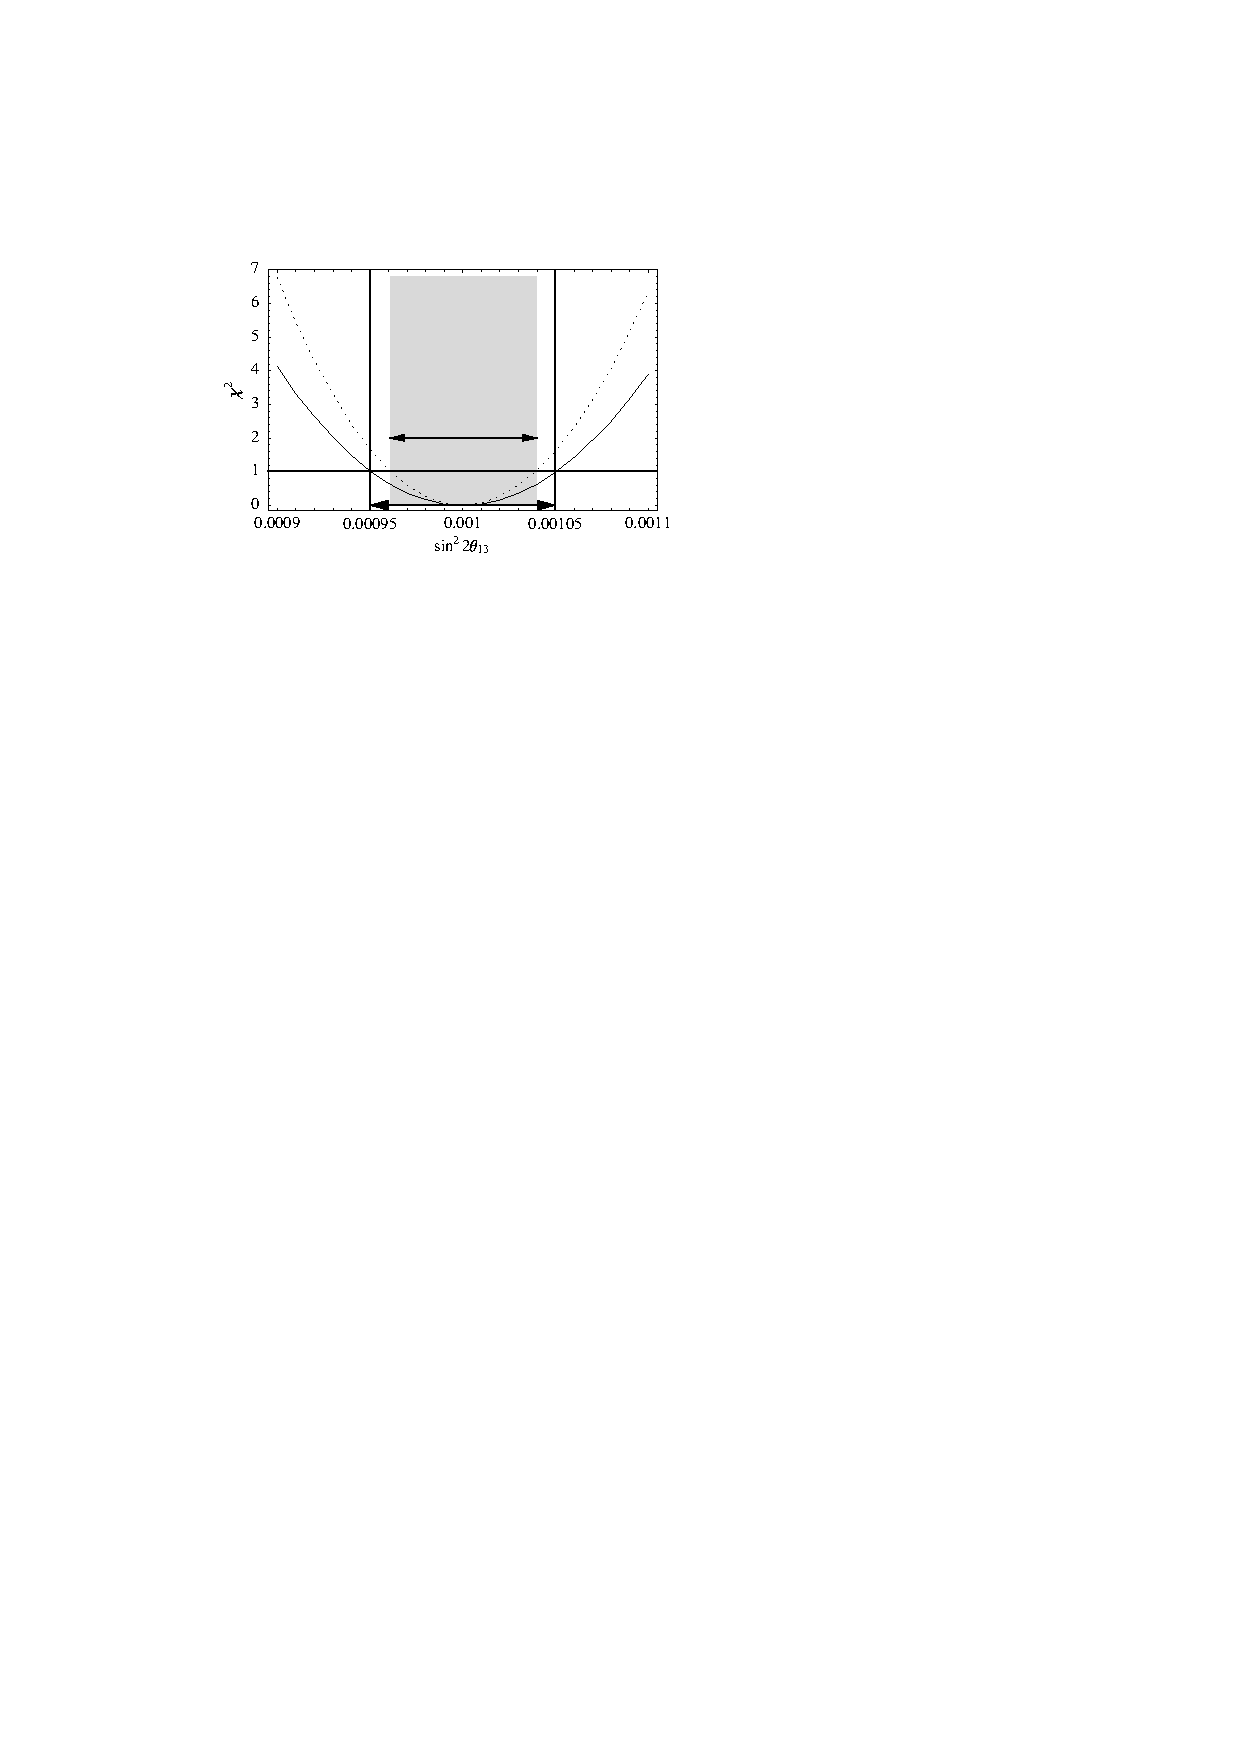
\includegraphics[width=6 cm]{fig/chi2_1dim.pdf} \hspace{0.5 cm}}
    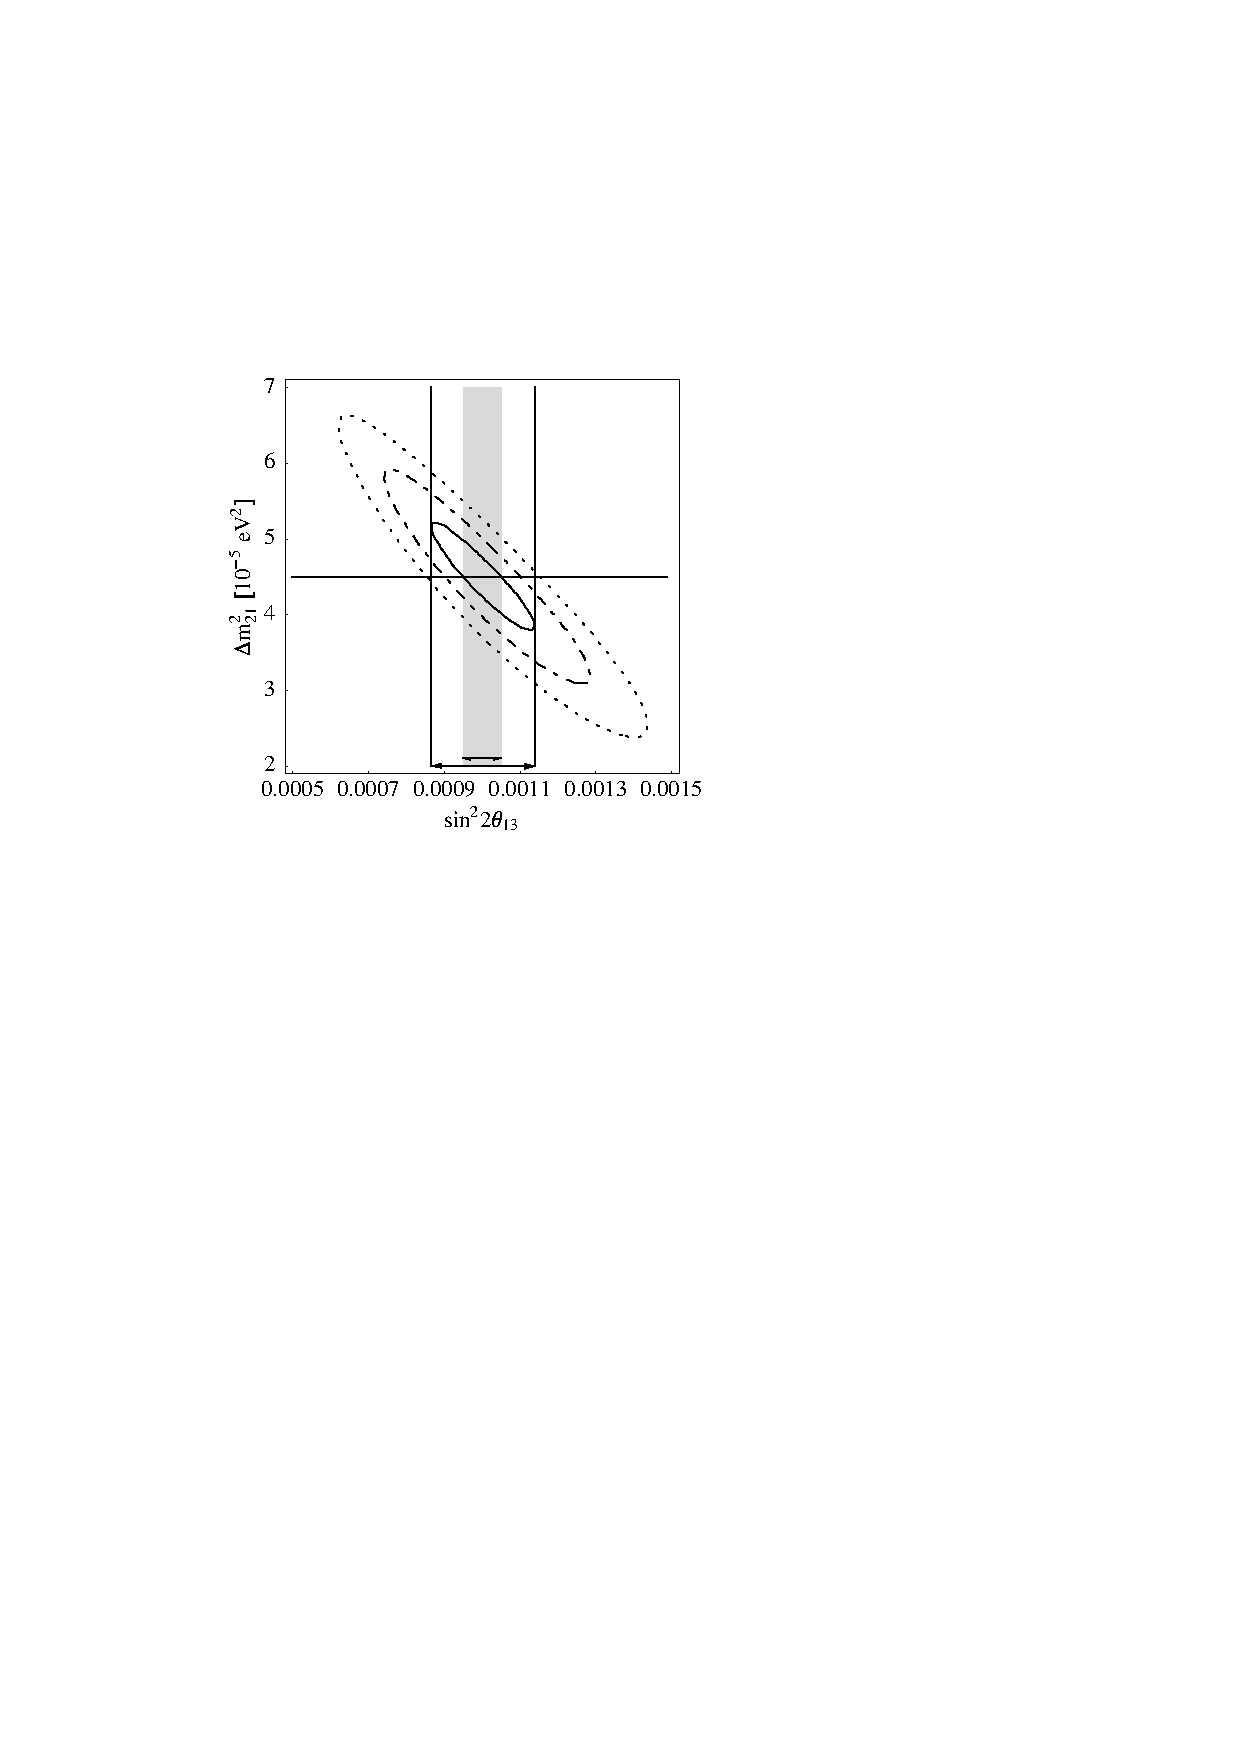
\includegraphics[width=5 cm]{fig/chi2_2dim.pdf}
  \end{figure}
  \begin{flushright}
    \reference{P. Huber, M. Lindner, W. Winter, Nucl. Phys. B645:3-48, 2002, hep-ph/0204352}
  \end{flushright}
\end{frame}



% =============================================================================
\section{Simulation of Future Oscillation Experiments}
% =============================================================================

% -----------------------------------------------------------------------------
\subsection{The R2D2 Setup}
% -----------------------------------------------------------------------------

\begin{frame}
  \frametitle{The $\bar{\nu}_e$ disappearance channel}

  \begin{figure}
    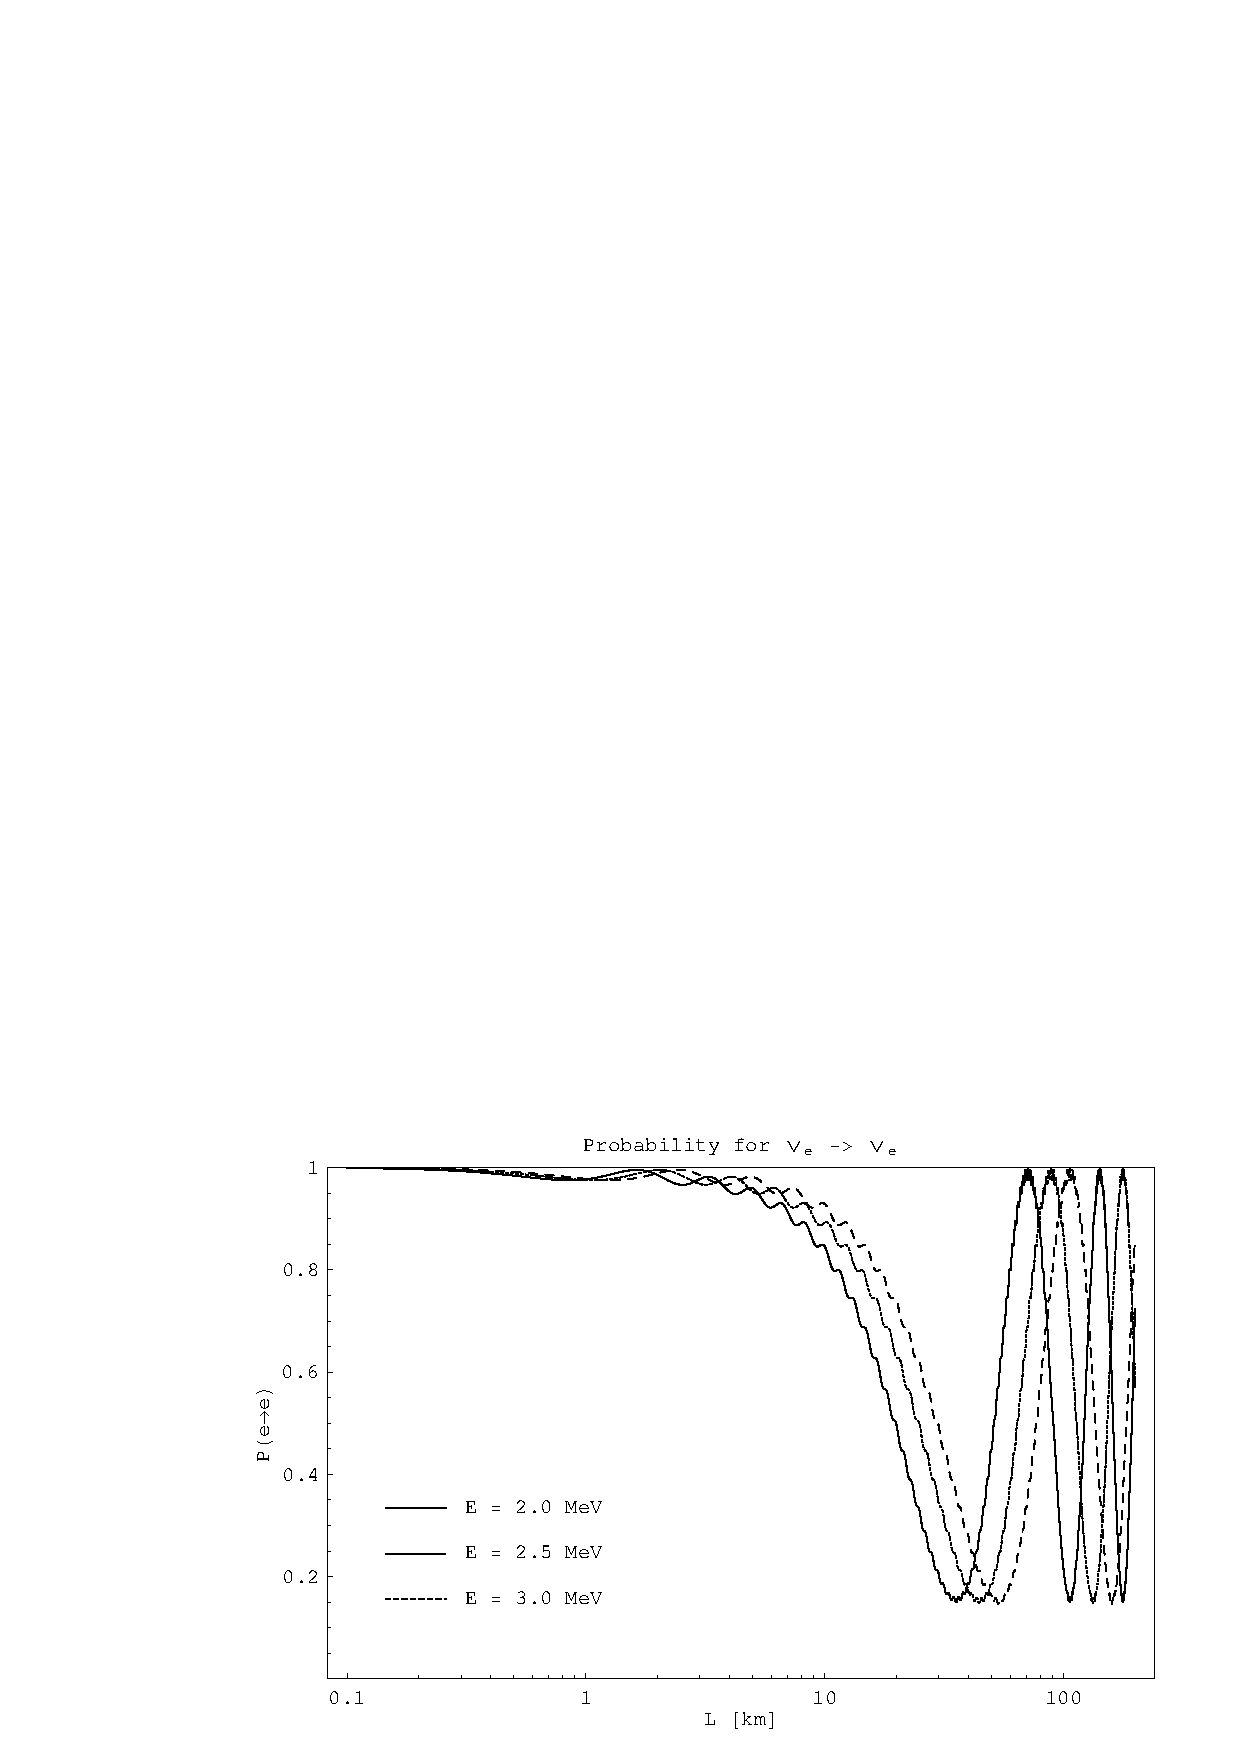
\includegraphics[width=12 cm]{fig/P_ee.pdf}
  \end{figure}
\end{frame}

\begin{frame}
  \frametitle{The R2D2 Setup}

  \begin{figure}
    \includegraphics[width=11 cm]{fig/R2D2_geometry.pdf}
  \end{figure}
  \begin{flushright}
    \reference{P. Huber, M. Lindner, T. Schwetz, JHEP 0502:029, 2005, hep-ph/0411166}
  \end{flushright}
  \begin{itemize}
    \item Near and far detectors $\longrightarrow$ Elimination of flux normalization error
    \item Two reactors $\longrightarrow$ Elimination of detector systematics
  \end{itemize}
\end{frame}

\begin{frame}
  \frametitle{The R2D2 Setup}

  \begin{figure}
    \includegraphics[height=7 cm]{fig/R2D2_s22th13.pdf}
  \end{figure}
  \begin{flushright}
    \reference{P. Huber, M. Lindner, T. Schwetz, JHEP 0502:029, 2005, hep-ph/0411166}
  \end{flushright}
\end{frame}


% -----------------------------------------------------------------------------
\subsection{Superbeams and Neutrino Factories}
% -----------------------------------------------------------------------------

\begin{frame}
  \frametitle{Superbeams}
  \begin{figure}
    \includegraphics[height=5 cm]{fig/cern_superbeam.jpg}
  \end{figure}
  \begin{flushright}
    \reference{J. Bouchez, CERN Courier 42, No. 5}
  \end{flushright}
  \begin{itemize}
    \item High neutrino energy $\longrightarrow$ Easy to detect
    \item $\nu_\mu$ beam with $\nu_e$, $\bar{\nu}_e$ and $\bar{\nu}_\mu$ contamination
          $\longrightarrow$ limited physics potential
  \end{itemize}
\end{frame}

\begin{frame}
  \frametitle{Neutrino Factories}
  \begin{figure}
    \vspace{-0.8 cm}
    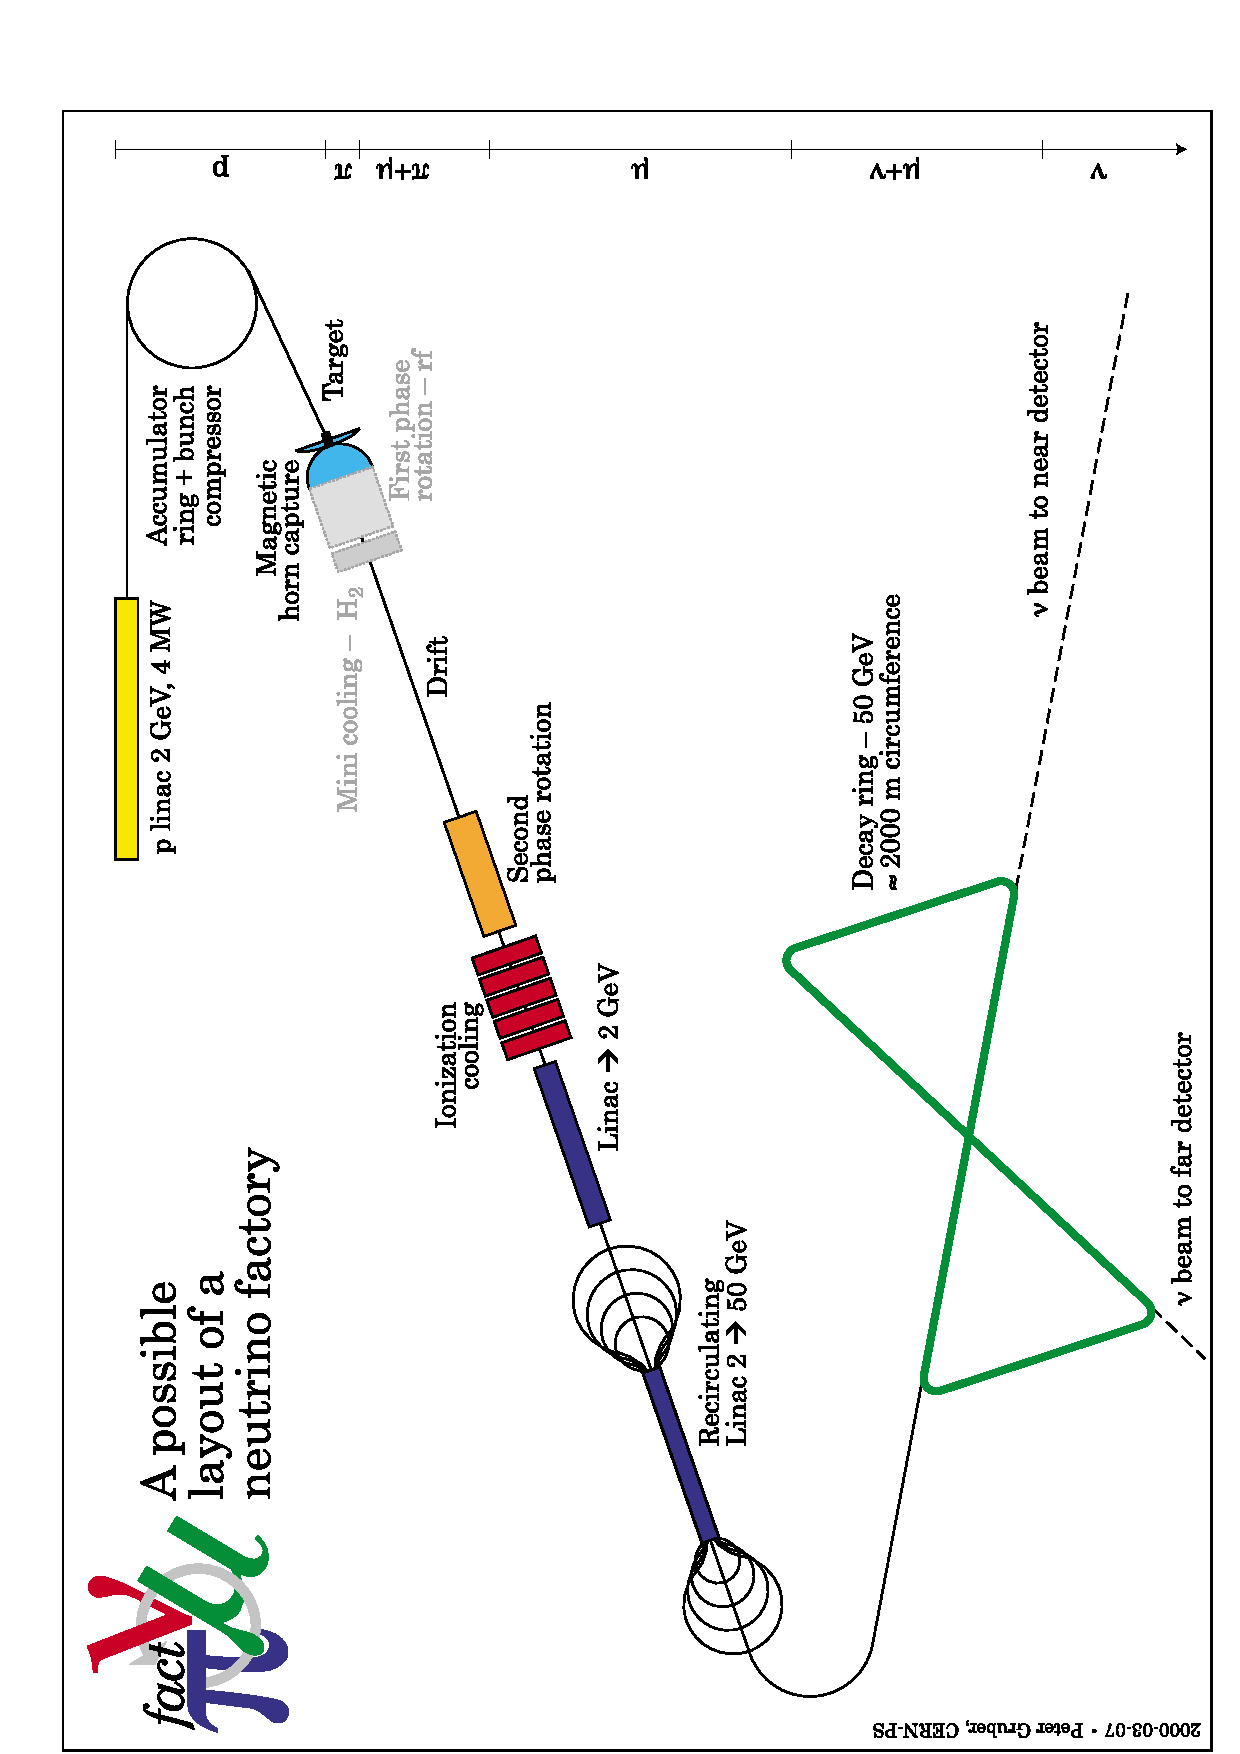
\includegraphics[height=8 cm,angle=270]{fig/cern_nufact.pdf}
    \vspace{-0.2 cm}
  \end{figure}
  \begin{itemize}
    \item High neutrino energy $\longrightarrow$ Easy to detect
    \item Long Baselines $\longrightarrow$ Exploiting matter effects
    \item Beam contains only $\nu_\mu$ and $\bar{\nu}_e$
          $\longrightarrow$ ``Wrong sign muon'' signature:
          Detection of $\mu^+$ indicates oscillation
  \end{itemize}
\end{frame}

\begin{frame}
  \frametitle{CP Violation in Superbeams and Neutrino Factories}
  \begin{figure}
    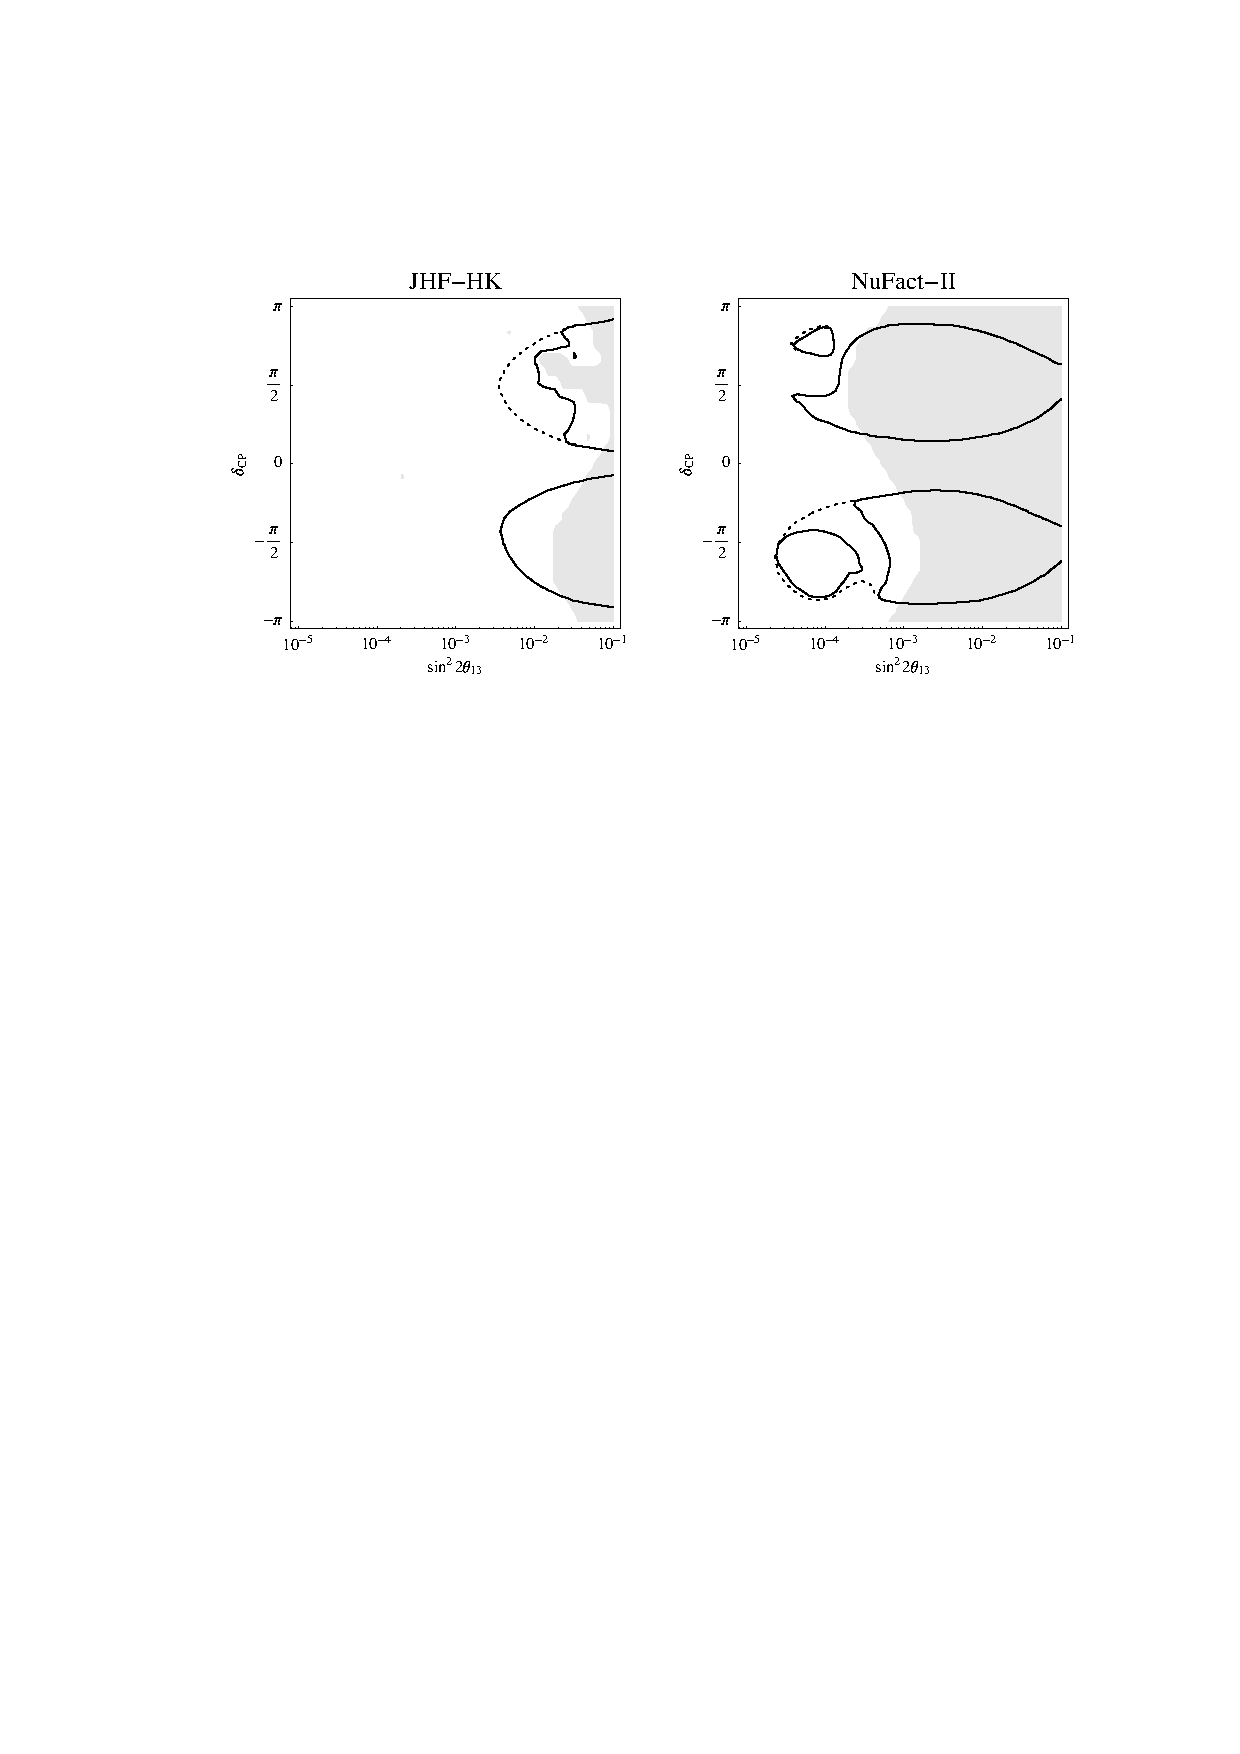
\includegraphics[height=4.5 cm]{fig/cpviolation.pdf}
  \end{figure}
  \begin{flushright}
    \reference{P. Huber, M. Lindner, W. Winter, Nucl. Phys. B645:3-48, 2002, hep-ph/0204352}
  \end{flushright}
  \begin{itemize}
    \item JHF-HK: $E_p$ = 50~GeV, L = 295 km, Target Power 4~MW, 1~Mt~Water \v{C}erenkov detector
    \item Nu-Fact II: $E_\mu$ = 50~GeV, L = 3000~km, Target Power: 4~MW,
                      $5 \cdot 10^{20} \frac{\mu}{\textnormal{year}}$, 50~kt~magnetized iron calorimeter
  \end{itemize}
\end{frame}

% -----------------------------------------------------------------------------
\subsection{Beta Beams}
% -----------------------------------------------------------------------------

\begin{frame}
  \frametitle{Beta Beams}
  \begin{figure}
    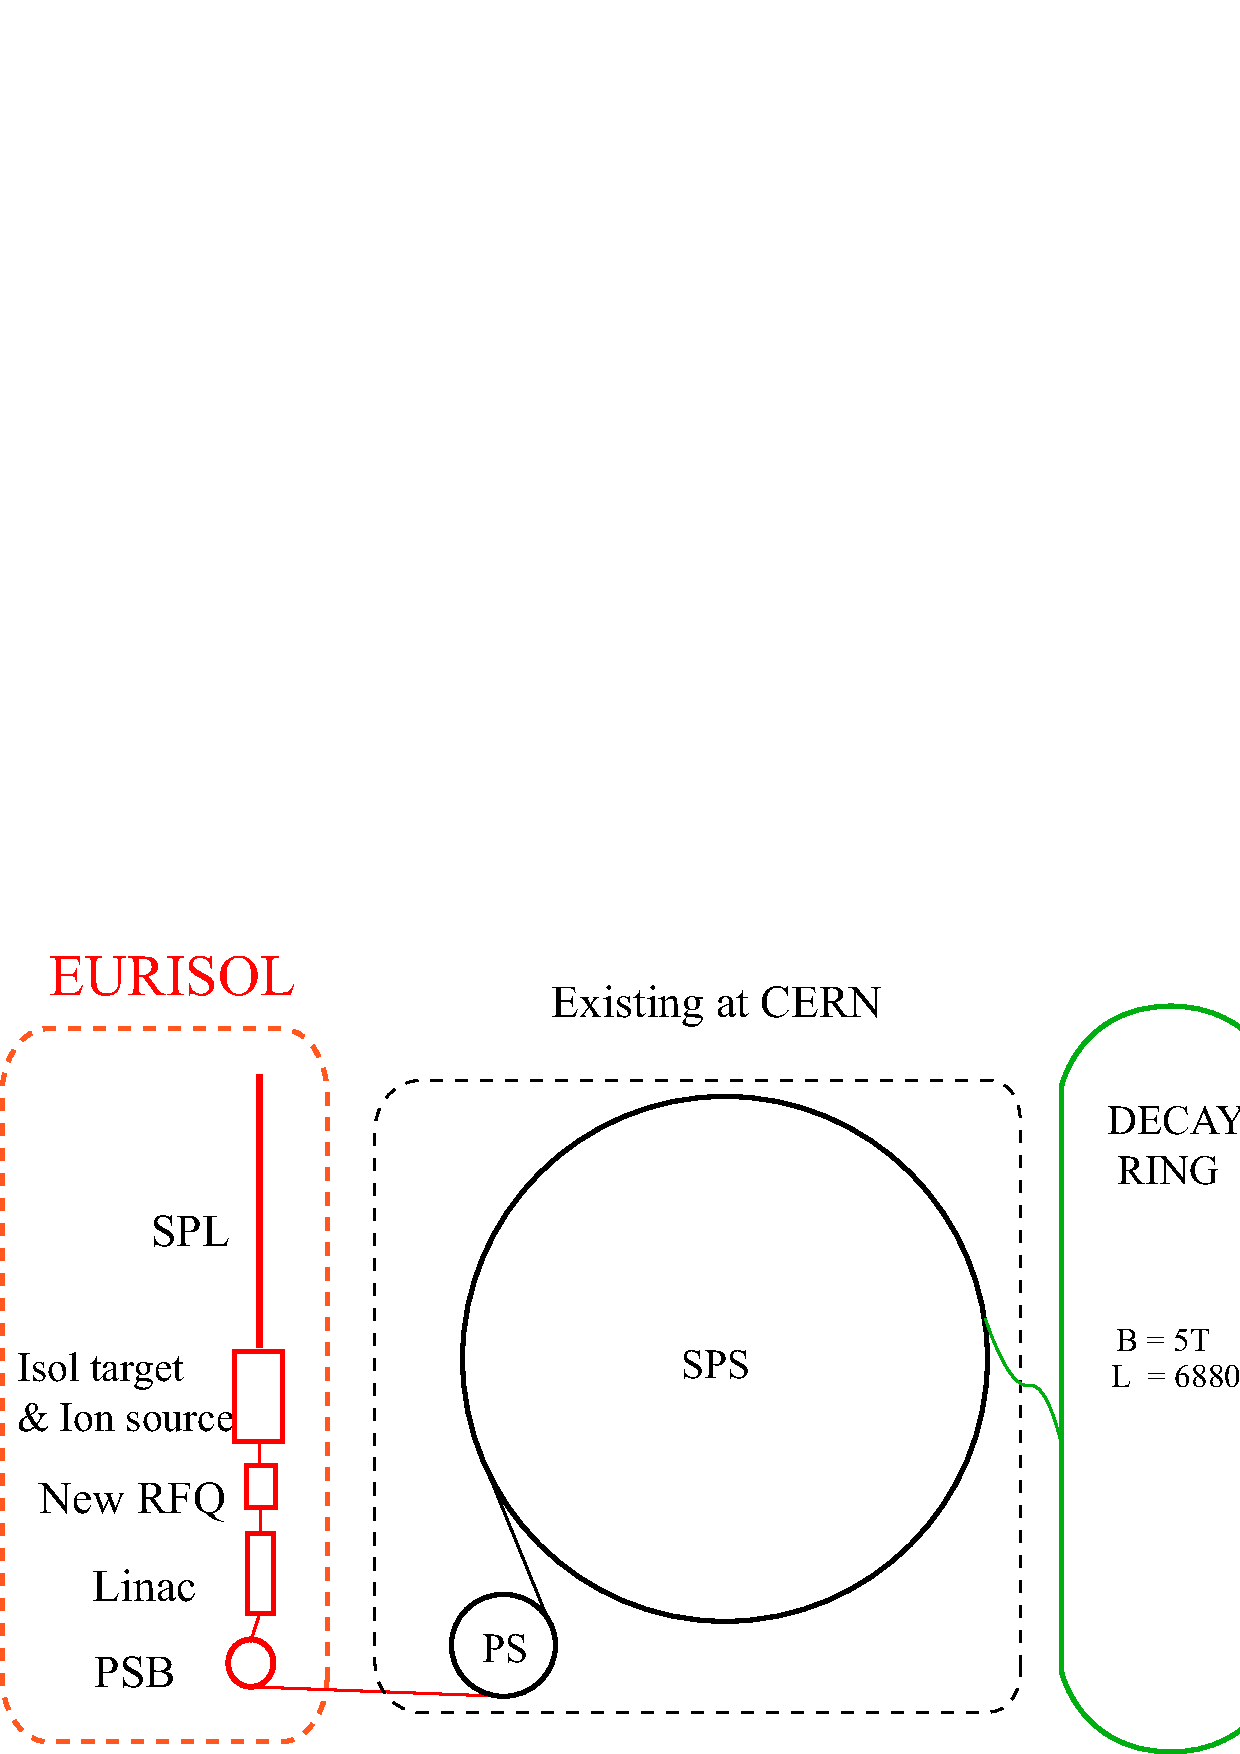
\includegraphics[height=5 cm]{fig/cern_betabeam.pdf}
  \end{figure}
  \begin{flushright}
    \reference{J. Bouchez, M. Lindroos, M. Mezzetto, AIP Conf. Proc. 721:37-47, 2004, hep-ex/0310059}
  \end{flushright}
  \begin{itemize}
    \item High neutrino energy $\longrightarrow$ Easy to detect
    \item Long Baselines $\longrightarrow$ Exploiting matter effects
    \item Pure $\nu_e$ or $\bar{\nu}_e$ beam
  \end{itemize}
\end{frame}

\begin{frame}
  \frametitle{Limitations of Neutrino Oscillation Experiments}
  \begin{figure}
    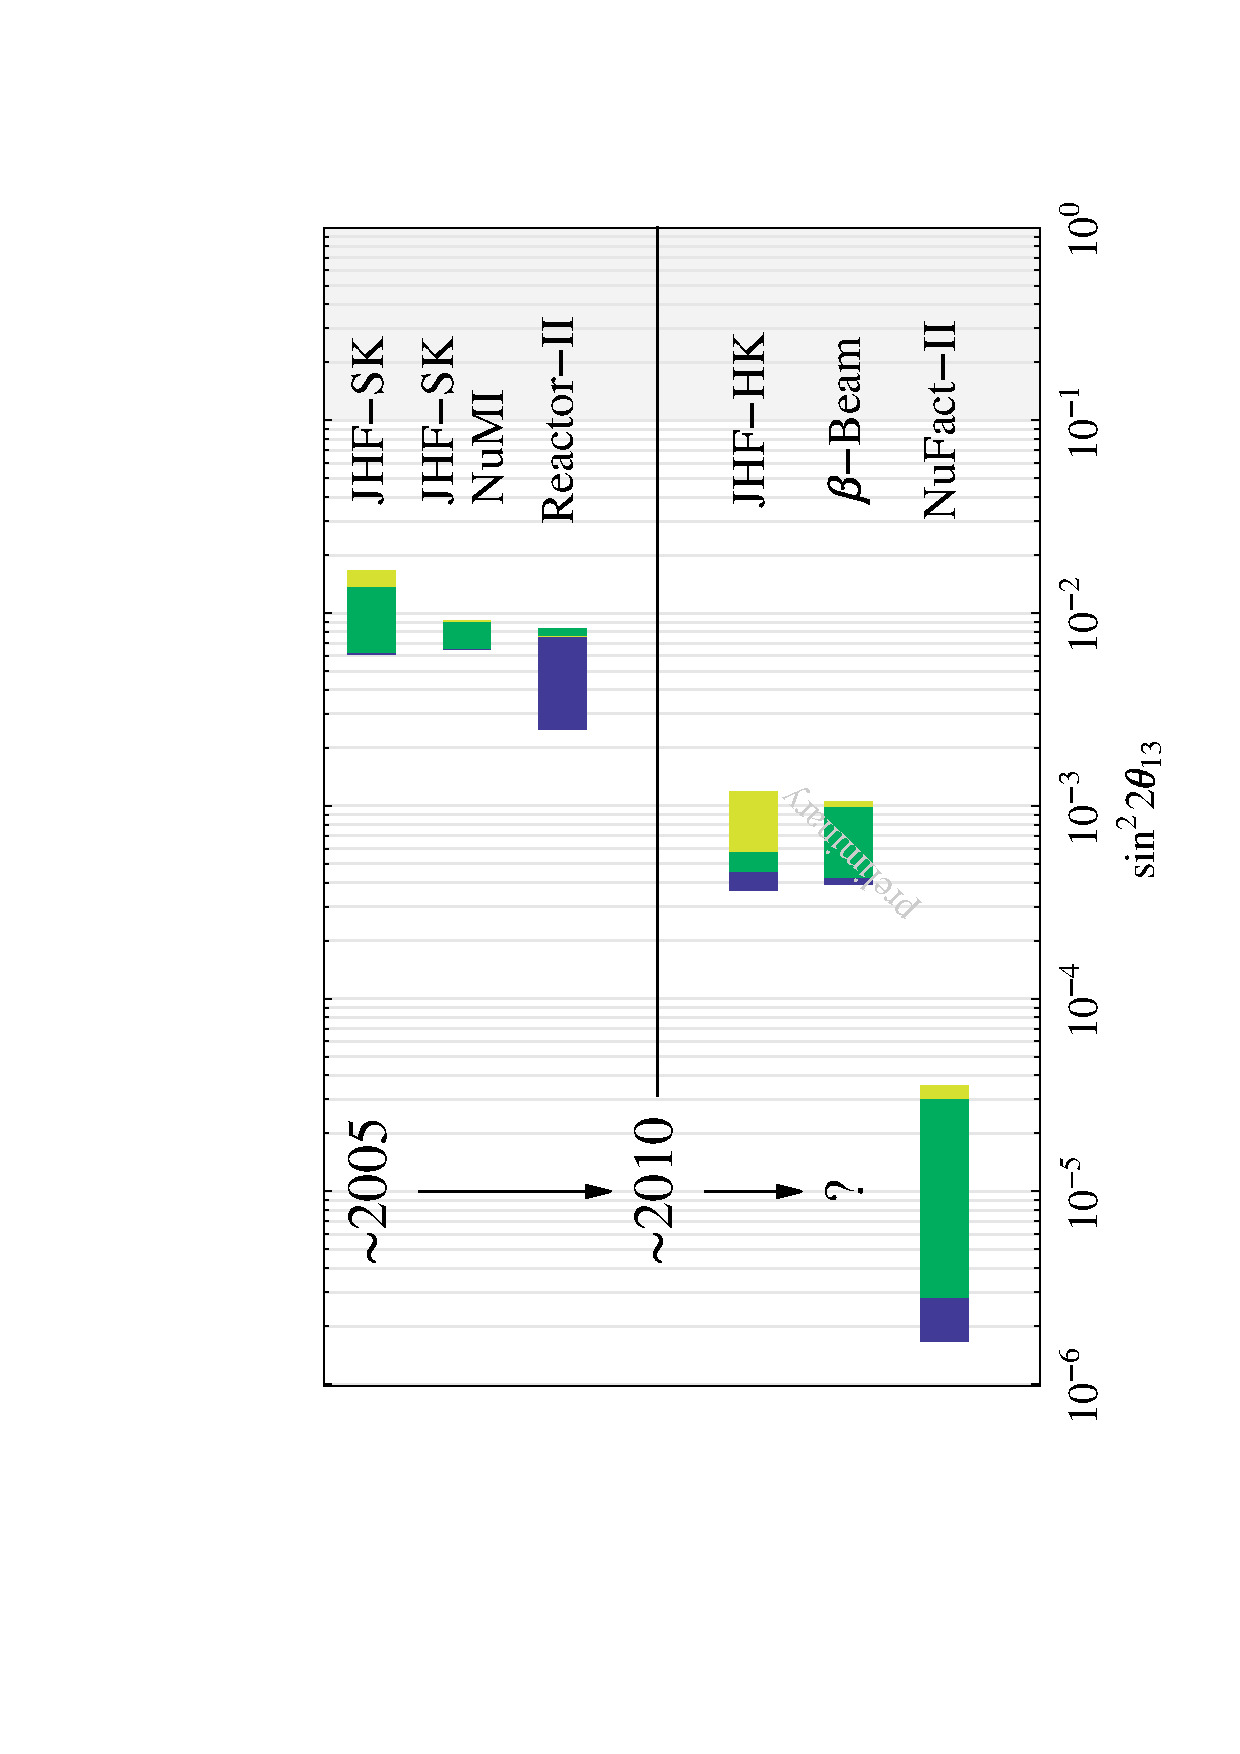
\includegraphics[height=5 cm]{fig/barplots.pdf}
  \end{figure}
  \begin{flushright}
    \reference{C. Albright et.al., physics/0411123}
  \end{flushright}
  \begin{itemize}
    \item Correlations: Sensitivity only to combination of parameters
    \item Degeneracies: Distinct regions in parameter space can explain the experiment
  \end{itemize}
\end{frame}

% =============================================================================
\section*{Conclusions}
% =============================================================================

\begin{frame}
  \frametitle{Conclusions}
  \begin{itemize}
    \item Neutrino oscillations are theoretically well understood and experimentally clearly
          verified.
    \item A precise determination of the oscillation parameters is desirable to achieve a deeper
          understanding of particle physics (flavour structure, $\ldots$).
    \item GLoBES is a tool for simulating future neutrino oscillation experiments and determine their
          physics potential.
    \item Nuclear reactors, Superbeams, Neutrino Factories and Beta Beams are excellent tools
          for solving many open questions.
  \end{itemize}
\end{frame}


\end{document}

